\documentclass{article}
\usepackage[utf8]{inputenc}
\usepackage{tikz}
\usepackage{karnaugh-map}
\usepackage{graphics}
\usepackage{hyperref}
\title{\textbf{Minimization of Boolean Functions using K-maps}}
\author{Syed Tabassum Nazeer}
\begin{document}
\maketitle
\begin{tableofcontents}
\begin{abstract}
This manual explains how to minimize the boolean functions using K-maps.
\end{abstract}
\section{COMPONENTS}
\begin{tabular}{|c||c||c|}
\hline
\textbf{component} & {value} & {quantity} \\
\hline
 \textbf{Breadboard}  &  &  1  \\
 \hline
 \textbf{Resistor}  & {220ohm} & {1} \\
 \hline
 \textbf{Arduino} & {Uno} & 1\\
 \hline
 \textbf{Sevensegment display} & {Common anode} & {1}\\
 \hline
 \textbf{Jumper wires} &   &  {20}\\
 \hline
\end{tabular}
%\centering{\textbf{Table}}
\\
\section{K-Maps}
The Karnaugh map or K-map is used for minimization or simplification of Boolean function either in Sum of Product(SOP) form or in Product of Sum(POS) form. A Karnaugh map is similar to a truth table because it presents all of the possible values of input variables and the resulting output for each value. Instead of being organized into columns and rows like a truth table, the Karnaugh map is an array of cells in which each cell represents a binary value of the input variables. The cells are arranged in a way so that simplification of a given expression is simply a matter of properly grouping the cells. Karnaugh maps can be used for expressions with two, three, four.and five variables. Another method, called the Quine-McClusky method can be used for higher numbers of variables. The number of cells in a Karnaugh map is equal to the total number of possible input variable combinations as is the number of rows in a truth table. For three variables, the number of cells is 23 = 8. For four variables, the number of cells is 24 = 16.
\section{Minimization}
The boolean fuction given in (1) is minimized using 3-variable K-maps.
Equation for F is
\begin{equation}
F= A'B'C'+A'BC'+A'BC+ABC'
\end{equation}
\\
the implicants 2,3 form a pair and results in the equation
\\
\begin{equation}
A'B
\end{equation}
\\
the implicants 2,6 form a pair and results in the equation
\\
\begin{equation}
B'C
\end{equation}
\\
the implicants 0,2 form a pair and results in the equation
\\
\begin{equation}
A'C'
\end{equation}
\centering
\begin{karnaugh-map}[4][2][1]
        \minterms{0,2,3,6}
        \maxterms{1,4,5,7}
        \implicant{3}{2}
        \implicant{2}{6}
    \end{karnaugh-map}
\\
Finally the minimized boolean function is represented by F' in (5)
\\
\section{Hardware}
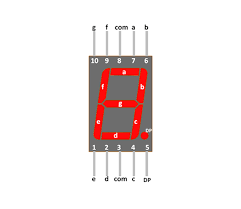
\includegraphics[scale=1.0]{sevenseg.png} 
\\
\begin{tabular}{|c|c|c|c|c|c|c||c|c|c|}
\hline
\textbf{Arduino} & 2 & 3 & 4 & 5 & 6 & 7 & 8 & com & dot\\
\hline
\textbf{Display} & {a} & {b} & {c} & {d} & {e} & {f} & {g} & {5V} & {GRD} \\
\hline
\end{tabular}
\newline
\newline
\\
Make the connections as per Table and execute the following program.
\end{tableofcontents}
\\
\\
\vspace{1cm}
\href{https://github.com/SyedTabassumNazeer/FWC/blob/main/main.cpp}{https://github.com/SyedTabassumNazeer/FWC/blob/main/main.cpp}
\end{document}
